\documentclass[twoside]{article}
% !TEX program = xelatex

\usepackage{cite}
\usepackage{listings}

\usepackage{fontspec}
\usepackage{titling}
\usepackage[utf8]{inputenc}
\usepackage{microtype} % Slightly tweak font spacing for aesthetics
\usepackage{graphicx}
\usepackage[round]{natbib}
\usepackage{hyperref}
\usepackage{placeins}

\usepackage[hmarginratio=1:1,top=32mm,columnsep=20pt,left=2cm,right=2cm]{geometry} % Document margins
\usepackage{multicol} % Used for the two-column layout of the document
\usepackage{wrapfig}
\usepackage[hang, small,labelfont=bf,up,textfont=it,up]{caption} % Custom captions under/above floats in tables or figures
\usepackage{booktabs} % Horizontal rules in tables
\usepackage{float} % Required for tables and figures in the multi-column environment - they need to be placed in specific locations with the [H] (e.g. \begin{table}[H])
\usepackage{hyperref} % For hyperlinks in the PDF

\usepackage{paralist} % Used for the compactitem environment which makes bullet points with less space between them

\usepackage{abstract} % Allows abstract customization
\renewcommand{\abstractnamefont}{\normalfont\bfseries} % Set the "Abstract" text to bold
\renewcommand{\abstracttextfont}{\normalfont\small\itshape} % Set the abstract itself to small italic text

\usepackage{titlesec} % Allows customization of titles
\renewcommand\thesection{\Roman{section}} % Roman numerals for the sections
\renewcommand\thesubsection{\Alph{subsection}}
\titleformat{\section}[block]{\large\scshape\centering}{\thesection.}{1em}{} % Change the look of the section titles
\titleformat{\subsection}[block]{\large}{\thesubsection.}{1em}{} % Change the look of the section titles

\graphicspath{{./images/}}

\usepackage{amsmath}
\usepackage{amssymb}

\newcommand{\bs}[1]{\mathbf{#1}}

\title{\vspace{-15mm}\fontsize{24pt}{10pt}\textbf{Bayesian optimization project report}}

\author{
  \large
  \textsc{Kenneth Blomqvist}\\[2mm]
  \texttt{kenneth.blomqvist@aalto.fi}\\[2mm]
}
\date{}

\newcommand{\norm}[1]{\left\lVert#1\right\rVert}

%----------------------------------------------------------------------------------------

% Set fonts

\newfontfamily\headingfont[]{Helvetica Bold}
\titleformat*{\section}{\LARGE\headingfont}
\titleformat*{\subsection}{\Large\headingfont}
\titleformat*{\subsubsection}{\large\headingfont}
\renewcommand{\maketitlehooka}{\headingfont}


\setmainfont[Scale=1.1]{Adobe Garamond Pro}
\linespread{1.1}

\begin{document}

\maketitle % Insert title

%----------------------------------------------------------------------------------------
%	ABSTRACT
%----------------------------------------------------------------------------------------

\begin{abstract}
  In this project I compare a bayesian optimization method to random search. The methods are compared on two different black-box optimization tasks. The results show that bayesian optimization outperforms random search on an easy low dimensional task. On the higher dimensional hyperparameter optimization task, both methods perform similarly.

\end{abstract}

%----------------------------------------------------------------------------------------
%	ARTICLE CONTENTS
%----------------------------------------------------------------------------------------

\begin{multicols}{2} % Two-column layout throughout the main article text

  \section{Introduction}
  \label{sec:introduction}
  
Often we want to optimize functions of which we do not have any knowledge but can do trial and error on. Examples of such functions include finding the best cookie recipe \citep{ml-cookies}, optimizing the hyperparameters of a machine learning algorithm and optimizing the parameters of an internet advertising campaign. In these cases, the function is very expensive to evaluate and therefore we want to spend as few evaluations as possible to find the best possible input while minimizing regret on the way.

One way to perform such black-box optimization is to randomly sample the input space and see what the output looks like. Once done with the exploration is done we simply select the best input parameters and use that going forward.

A more sophisticated way to approach the problem is to use bayesian optimization. In bayesian optimization we start with a few observations of the function inputs and corresponding outputs. We model the actual function with a gaussian process. Using our model of the function we make educated guesses to select inputs to try next. \citep{bayesian-opt}

In this project I implement a simple random optimization scheme and a bayesian optimization algorithm. I compare the performance of the two approaches on two different tasks. In the first task I try to find the optimal input for a randomly initialized polynomial linear regression function with random weights. In the second task I try to find the optimal hyperparameters for a convolutional neural network model operating on the CIFAR-10 dataset.

%%% Local Variables:
%%% mode: latex
%%% TeX-master: "report"
%%% End:


  \section{Methods}
  \label{sec:methods}
  
In this section I present the main methods used in this project.

\subsection{Black-box optimization}

In black-box optimization we are interested in finding the optimal input to a function without knowing much about the function. Our function takes $D$-dimensional input and outputs a scalar value. $f(\bs{x}): \mathbb{R}^D \mapsto \mathbb{R}$. We are trying to solve the equation: \[
    argmax_{\bs{x} \in R^D} f(\bs{x})
    \]
The input vector $\bs{x}$ might have some constraints on each of the dimensions. The different input variables might be integers in some cases.

The optimizer is given a budget which is the maximum number of times the optimization routine is allowed to evaluate the function. Once these evaluations have been spent we select the best input and that is the output of the optimization.

We assume that the function $f$ is L-lipschitz. What this means is that we assume that the function is roughly continuous. The observations of the outputs of the function might contain some unknown amount of noise.

\subsection{Random optimization}

This is the naive monte carlo approach to solve the problem.

We sample points from the input space from a uniform distribution over the entire input space. We return the input that produced the best output.

\subsection{Bayesian optimization}

In bayesian optimization we start out with a few random observations selected as in random optimization. Next we fit a gaussian process to the data and select the next points in the input space to sample using an acquisition function.

The gaussian process $GP(m(x), k(x, x'))$ has a mean function $m(x)$ along with a kernel function $k(x, x')$. We normalize our observations to have unit variance and zero mean. Thus it is natural to use the constant zero function as the prior mean function.

Once the gaussian process is fitted to the data we can make predictions on the output of the underlying function. Gaussian processes allow us to compute uncertainty estimates on predictions. Using the predictions and corresponding uncertainty estimates we can make informed guesses on which areas of the input space to try next. This function on the predictions and uncertainties is called the acquisition function.

In my experiments I used the matern52 kernel function with automatic relevance determination. Automatic relevance determination learns individual parameters for each dimension.

\subsubsection{The acquisition function}

The acquisition function tells us which point to try next. It takes as input the mean prediction over the input space along with the variance. There are many different types of acquisition functions such as probability of improvement, expected improvement and upper confidence bound. Some strategies even combine several of these functions. \citep{bayesian-opt}

To keep things simple I decided to use the upper confidence bound acquisition function.

\begin{align}
    a_{UCB}(\bs{x}; {\bs{\bs{x}_n, y_n}, \bs{\theta}}) = \mu(\bs{x}; {\bs{\bs{x}_n, y_n}, \bs{\theta}}) + \kappa * \sigma(\bs{x}; {\bs{\bs{x}_n, y_n}, \bs{\theta}})
\end{align}

$\mu$ is the mean function of our fitted gaussian process and $\sigma$ is the standard deviation of our prediction at point $\bs{x}$. $\kappa$ is a hyperparameter which determines how much we explore vs. exploit. I set this parameter to $2.5$.

Essentially this acquisition strategy uses the `optimism in the face of uncertainty' heuristic to explore the input space. If we are not sure about an area in the input space we assume the output will be at the best edge of our uncertainty estimate. That is, we are very optimistic about the world.

To maximize the acquisition function I used the L-BFGS-B algorithm.


%%% Local Variables:
%%% mode: latex
%%% TeX-master: "report"
%%% End:


  \section{Experiments}
  \label{sec:experiments}
  
In this project I was primarily interested in these questions:
\begin{itemize}
    \item Does it always make sense to use bayesian optimization over random search?
    \item Does bayesian optimization make sense in a high dimensional and low sample regime?
\end{itemize}

To investigate these questions I implemented two different experiments. In the first one I try to find the optimal input for a randomly generated polynomial regression functio. In the second experiment I try to find the hyperparameters for a convolutional neural network model that yield the highest test accuracy on the CIFAR-10 dataset.

\subsection{Random polynomial regression}

In this experiment I initialize a polynomial regression function with added noise
\[
    y = \boldsymbol{w^T\phi(x)} + \epsilon
\]
where x is two dimensional and $\phi$ expands the input to include powers from 0 to 6.
\[
    \boldsymbol{\phi(x)} = \begin{bmatrix}
        x_0^0 \\
        x_0^1 \\
        \vdots \\
        x_0^6 \\
        x_1^0 \\
        \vdots \\
        x_1^6
    \end{bmatrix}
\]

The weights were drawn randomly for each experiment such that each weight was drawn from a uniform distribution with minimum -0.01 and maximum 0.01. The noise $\epsilon$ was drawn from from a normal distribution with zero mean and scale 10.

$x_0$ and $x_1$ are restricted to be in the range $[-10, 10]$. Each optimizer was given a function evaluation budget of 25 evaluations. The goal is to find the input that yields the highest regression value without having access to the function itself.

This problem is more of a toy problem and the point was to validate each. It should be fairly easy to solve as the function is very smooth. However, the function might have several optima of which only one is global.

I ran this experiment 25 times with both methods and analyze the the results section \ref{sec:results}.

\subsection{CNN hyperparameter tuning}

I implemented a ResNet \citep{resnet} type architecture to classify images from the CIFAR-10 dataset \citep{cifar}. The CIFAR-10 dataset contains 50 000 training examples and 10 000 test examples.

I implemented the network using the Pytorch software package \citep{pytorch}. The network was trained for 50 epochs using stochastic gradient descent with momentum.

The layers in the model were as such:
\begin{itemize}
    \item 1 x 3x3 conv layer with stride 1 and 64 feature maps
    \item $layers_1$ x 3x3 conv layers with stride 1 and 64 feature maps
    \item $layers_2$ x 3x3 conv layers with stride 2 and 128 feature maps
    \item $layers_3$ x 3x3 conv layers with stride 2 and 256 feature maps
    \item $layers_4$ x 3x3 conv layers with stride 2 and 512 feature maps
    \item Average pooling with stride 1 and size 4x4.
    \item A fully connected layer followed by a softmax activation
\end{itemize}
\vfill

Table \ref{hyperparameters} shows the hyperparameters that were included in the optimization as well as the ranges allowed.

\begin{center}
    \begin{tabular}{ c | c | c }
    \bf{Parameter} & \bf{Minimum} & \bf{Maximum} \\
    \hline
    \bf{SGD momentum} & 0 & 1.0 \\
    \bf{Learning rate} & 0.0001 & 0.5 \\
    \bf{Layers 1} & 1 & 8 \\
    \bf{Layers 2} & 1 & 8 \\
    \bf{Layers 3} & 1 & 8 \\
    \bf{Layers 4} & 1 & 8 \\
    \bf{Conv dropout} & 0 & 0.8 \\
    \bf{Fully connected dropout} & 0 & 0.8 \\
    \end{tabular}
    \captionof{table}{Table of hyperparameters.}
    \label{hyperparameters}
\end{center}

The conv dropout is the amount of dropout applied after each of the convolutional blocks sharing the same feature map count. The fully connected dropout is applied before the average pooling layer.


%%% Local Variables:
%%% mode: latex
%%% TeX-master: "report"
%%% End:


  \section{Results}
  \label{sec:results}
  
This section presents the results obtained in the experiments.

\subsection{The random regression}

I ran the regression input optimization experiment detailed in section \ref{sec:experiments} 25 times. Each experiment was initialized with different random weights on the regression function. For each experiment both optimization methods were allowed to evaluate the function 25 times.

\begin{center}
    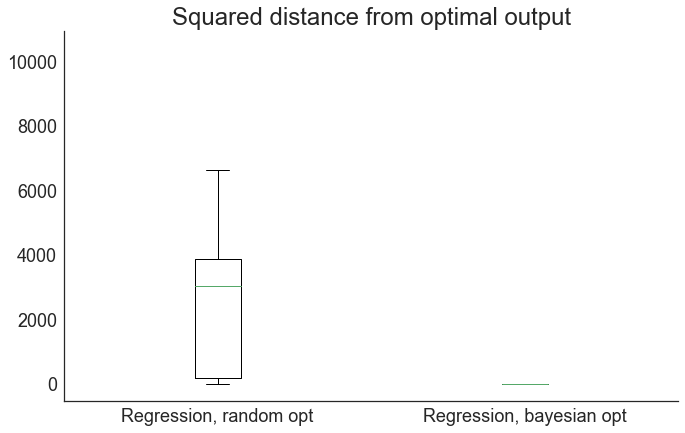
\includegraphics[width=\linewidth]{random_regression.png}
    \captionof{figure}{Squared distance and confidence intervals from the optimal output for both methods. }
    \label{image:random-regression}
\end{center}

\begin{center}
    \begin{tabular}{ c | c | c }
    \bf{Optimization method} & \bf{mean} & \bf{variance} \\
    \hline
    \bf{Random search} & 2925.13 & 8098738.45 \\
    \bf{Bayesian optimization} & 41.42 & 19133.35 \\
    \end{tabular}
    \captionof{table}{Mean squared distance from the optimal output across all 25 runs of the experiments. }
    \label{table:random-regression}
\end{center}

\subsection{Hyperparameter optimization}

Due to the high computational cost of training neural networks, I was only able to run the experiment once for each method. Each method was given 25 function evaluations.

\begin{center}
    \begin{tabular}{ c | c | c }
    \bf{Method} & \bf{best test acc.} & \bf{variance in acc.} \\
    \hline
    \bf{Random search} & 31.23 & 113.98 \\
    \bf{Bayesian optimization} & 31.16 & 98.88 \\
    \end{tabular}
    \captionof{table}{Mean across experiments from the squared distance from the optimum output with the best value found. }
    \label{table:hyperparameter-opt}
\end{center}

The full outputs for the experiments can be seen in appendix \ref{appendix:cnn}



%%% Local Variables:
%%% mode: latex
%%% TeX-master: "report"
%%% End:


  \section{Discussion}
  \label{sec:discussion}
  
As we saw in the results section \ref{sec:results} bayesian optimization performs very well on the random regression optimization task. It completely blows random search out of the water. In this task the function to optimize was very smooth and there was only a small amount of noise. Bayesian optimization finds the global optimum almost every time.

Random search explores the space well, but has very high variance as shown in the regression task results.

For optimizing the hyperparameters, the methods performed very similarly. Bayesian optimization explores the input space very well but since the input space is so large, maximizing the acquisition function degrades to random search as there is so much uncertainty. It would be interesting to see if it would perform better if there were fewer dimensions.

What I learned about optimizing hyperparameters was that there appears to be very large areas in the hyperparameter space that work well. Supprisingly the depth of the model had a very small effect. The learning rate was clearly an important parameter. The best outputs had a learning rate of 0.05-0.3. Momentum did not seem to matter that much. A lot of the good results seem to have high dropout rates. However, there are also some runs with low dropout rates that did well.

It's hard to tell how much noise there is in the training process or why some hyperparameters lead to very bad results. It would require more exploration of the parameter space.

Before running the hyperparameter optimization experiment I ran it a couple of times to make sure everything works. I was able to achieve a test accuracy of 29.63 by selecting the parameters based on my experience and intuition.

I would like to explore ways of automatically trying different kernel functions. Since we do not know anything about the functions we are optimizing, it would be desirable to not have to make any assumptions on the structure of function we are optimizing. The kernel that maximizes likelihood across many fits of the GP could be selected automatically.

To conclude, it seems that bayesian optimization is a very powerful technique. Bayesian optimization has significant advantages over random search with minimal drawbacks. However, it is not bliss. As the size of the input space increases we have acquire exponentially more samples to gain certainty about the behaviour of our function. I will be sure to use bayesian optimization in the future, but I will at least try to prune the search space using reasoning, theory and intuition to the farthest extent possible.



%%% Local Variables:
%%% mode: latex
%%% TeX-master: "report"
%%% End:



  %	REFERENCE LIST
  %----------------------------------------------------------------------------------------

  \bibliographystyle{plainnat}
  \bibliography{references}

\end{multicols} % One-column layout for the appendices
\pagebreak

\section{Appendix A: CNN experiment data}

\FloatBarrier
\subsection{Random optimization}

\begin{table}[h]
    \centering
    \small
    \begin{tabular}{@{}lllllll@{}}
    \toprule
    \textbf{Attempt} & \textbf{lr}       & \textbf{momentum} & \textbf{layers} & \textbf{conv\_dropout} & \textbf{fc\_dropout} & \textbf{Output} \\ \midrule
    11               & {[} 0.09638509{]} & {[} 0.39767684{]} & {[}6 5 2 1{]}   & {[} 0.45680685{]}      & {[} 0.51026919{]}    & 31.2316         \\
    22               & {[} 0.31908397{]} & {[} 0.15333848{]} & {[}1 6 4 1{]}   & {[} 0.62556677{]}      & {[} 0.49306316{]}    & 31.0147         \\
    21               & {[} 0.14137594{]} & {[} 0.61294809{]} & {[}4 1 7 1{]}   & {[} 0.34225011{]}      & {[} 0.34270592{]}    & 30.9375         \\
    8                & {[} 0.3942071{]}  & {[} 0.26554666{]} & {[}2 4 5 3{]}   & {[} 0.20878318{]}      & {[} 0.18481234{]}    & 30.75           \\
    16               & {[} 0.04582328{]} & {[} 0.62336012{]} & {[}1 6 1 2{]}   & {[} 0.44105995{]}      & {[} 0.0560652{]}     & 30.6434         \\
    17               & {[} 0.26380973{]} & {[} 0.74276483{]} & {[}6 5 5 4{]}   & {[} 0.18429025{]}      & {[} 0.40659803{]}    & 30.3346         \\
    5                & {[} 0.29414724{]} & {[} 0.1975509{]}  & {[}1 2 4 5{]}   & {[} 0.62665158{]}      & {[} 0.33003107{]}    & 30.3235         \\
    2                & {[} 0.06102909{]} & {[} 0.02738759{]} & {[}3 5 2 2{]}   & {[} 0.11230955{]}      & {[} 0.15848119{]}    & 30.0257         \\
    14               & {[} 0.27508892{]} & {[} 0.57838961{]} & {[}3 7 7 3{]}   & {[} 0.72270362{]}      & {[} 0.45894359{]}    & 27.9338         \\
    20               & {[} 0.45423093{]} & {[} 0.57006666{]} & {[}7 7 1 6{]}   & {[} 0.65039598{]}      & {[} 0.231808{]}      & 27.7463         \\
    6                & {[} 0.48291776{]} & {[} 0.62402999{]} & {[}1 5 2 3{]}   & {[} 0.63142346{]}      & {[} 0.08258081{]}    & 27.6103         \\
    0                & {[} 0.2915307{]}  & {[} 0.72032449{]} & {[}2 4 6 1{]}   & {[} 0.07387088{]}      & {[} 0.14900817{]}    & 27.1912         \\
    18               & {[} 0.3957367{]}  & {[} 0.04930424{]} & {[}3 6 6 5{]}   & {[} 0.02096879{]}      & {[} 0.02264519{]}    & 26.864          \\
    4                & {[} 0.08528128{]} & {[} 0.27304997{]} & {[}3 2 1 7{]}   & {[} 0.47445241{]}      & {[} 0.53732328{]}    & 26.5956         \\
    1                & {[} 0.32725419{]} & {[} 0.39676747{]} & {[}3 5 7 6{]}   & {[} 0.5481756{]}       & {[} 0.1635618{]}     & 26.4816         \\
    23               & {[} 0.48200388{]} & {[} 0.65432377{]} & {[}4 1 2 3{]}   & {[} 0.2886518{]}       & {[} 0.21971612{]}    & 25.0037         \\
    10               & {[} 0.43003094{]} & {[} 0.79240359{]} & {[}4 6 4 6{]}   & {[} 0.10997976{]}      & {[} 0.11142108{]}    & 24.7132         \\
    24               & {[} 0.4630229{]}  & {[} 0.15213716{]} & {[}4 3 4 7{]}   & {[} 0.29690712{]}      & {[} 0.04001447{]}    & 24.7022         \\
    9                & {[} 0.2333291{]}  & {[} 0.94993814{]} & {[}6 4 1 1{]}   & {[} 0.61238808{]}      & {[} 0.03627658{]}    & 23.5662         \\
    3                & {[} 0.09970779{]} & {[} 0.96826158{]} & {[}6 7 2 2{]}   & {[} 0.6920162{]}       & {[} 0.66331753{]}    & 6.47059         \\
    7                & {[} 0.27609803{]} & {[} 0.9085955{]}  & {[}7 6 5 4{]}   & {[} 0.01549357{]}      & {[} 0.54306843{]}    & 3.67647         \\
    12               & {[} 0.43685519{]} & {[} 0.69020459{]} & {[}2 1 3 5{]}   & {[} 0.21594231{]}      & {[} 0.71670897{]}    & 3.67647         \\
    13               & {[} 0.28599721{]} & {[} 0.96484005{]} & {[}3 4 2 3{]}   & {[} 0.09179678{]}      & {[} 0.75959141{]}    & 3.67647         \\
    15               & {[} 0.49856512{]} & {[} 0.61714491{]} & {[}5 7 1 7{]}   & {[} 0.70875368{]}      & {[} 0.28581581{]}    & 3.67647         \\
    19               & {[} 0.37691909{]} & {[} 0.86002795{]} & {[}6 1 7 6{]}   & {[} 0.22265507{]}      & {[} 0.18689802{]}    & 3.67647         \\ \bottomrule
    \end{tabular}
\end{table}

\FloatBarrier

\subsection{Bayesian optimization}

\begin{table}[h]
    \centering
    \small
    \begin{tabular}{@{}lllllll@{}}
    \toprule
    \textbf{Attempt} & \textbf{lr}       & \textbf{momentum} & \textbf{layers} & \textbf{conv\_dropout} & \textbf{fc\_dropout} & \textbf{Output} \\ \midrule
    10               & {[} 0.05405183{]} & {[} 0.51805344{]} & {[}5 7 5 2{]}   & {[} 0.52639126{]}      & {[} 0.61087903{]}    & 31.1618         \\
    13               & {[} 0.07226851{]} & {[} 0.27007622{]} & {[}6 6 8 4{]}   & {[} 0.01398236{]}      & {[} 0.6524798{]}     & 31.0074         \\
    2                & {[} 0.06102909{]} & {[} 0.02738759{]} & {[}3 5 2 2{]}   & {[} 0.11230955{]}      & {[} 0.15848119{]}    & 30.6324         \\
    20               & {[} 0.21347942{]} & {[} 0.69142559{]} & {[}4 5 3 5{]}   & {[} 0.34429719{]}      & {[} 0.50676947{]}    & 30.1581         \\
    15               & {[} 0.25836809{]} & {[} 0.41800128{]} & {[}6 7 7 6{]}   & {[} 0.74964996{]}      & {[} 0.75580912{]}    & 29.3566         \\
    17               & {[} 0.45357083{]} & {[} 0.00626705{]} & {[}4 7 5 7{]}   & {[} 0.03459003{]}      & {[} 0.41876539{]}    & 28.864          \\
    21               & {[} 0.36376611{]} & {[} 0.08088232{]} & {[}5 6 5 7{]}   & {[} 0.75893059{]}      & {[} 0.31979356{]}    & 28.7831         \\
    6                & {[} 0.15850852{]} & {[} 0.08410233{]} & {[}4 2 6 6{]}   & {[} 0.28245794{]}      & {[} 0.14448219{]}    & 28.1176         \\
    1                & {[} 0.32725419{]} & {[} 0.39676747{]} & {[}3 5 7 6{]}   & {[} 0.5481756{]}       & {[} 0.1635618{]}     & 27.75           \\
    8                & {[} 0.32633348{]} & {[} 0.2548282{]}  & {[}7 5 5 5{]}   & {[} 0.52830732{]}      & {[} 0.50010018{]}    & 27.5221         \\
    0                & {[} 0.2915307{]}  & {[} 0.72032449{]} & {[}2 4 6 1{]}   & {[} 0.07387088{]}      & {[} 0.14900817{]}    & 27.511          \\
    9                & {[} 0.3489775{]}  & {[} 0.52222017{]} & {[}5 8 6 5{]}   & {[} 0.68365825{]}      & {[} 0.09161118{]}    & 27.3346         \\
    24               & {[} 0.13252658{]} & {[} 0.32492428{]} & {[}8 3 5 4{]}   & {[} 0.14121815{]}      & {[} 0.02221327{]}    & 27.2684         \\
    12               & {[} 0.3071959{]}  & {[} 0.03943446{]} & {[}2 3 6 6{]}   & {[} 0.22768015{]}      & {[} 0.27684347{]}    & 26.5294         \\
    4                & {[} 0.48354893{]} & {[} 0.113411{]}   & {[}4 1 5 2{]}   & {[} 0.20076923{]}      & {[} 0.34119436{]}    & 25.9596         \\
    19               & {[} 0.09955684{]} & {[} 0.72595784{]} & {[}8 1 2 2{]}   & {[} 0.73534641{]}      & {[} 0.78932408{]}    & 24.6728         \\
    3                & {[} 0.0370019{]}  & {[} 0.91873344{]} & {[}4 8 2 2{]}   & {[} 0.10806333{]}      & {[} 0.40452973{]}    & 24.4412         \\
    11               & {[} 0.41192775{]} & {[} 0.1582323{]}  & {[}7 2 2 3{]}   & {[} 0.70909899{]}      & {[} 0.75224333{]}    & 24.1471         \\
    14               & {[} 0.00294731{]} & {[} 0.01024019{]} & {[}5 8 3 5{]}   & {[} 0.02722457{]}      & {[} 0.64976272{]}    & 21.0221         \\
    22               & {[} 0.43277007{]} & {[} 0.83744782{]} & {[}4 5 1 2{]}   & {[} 0.01629748{]}      & {[} 0.08255292{]}    & 20.2206         \\
    5                & {[} 0.45273732{]} & {[} 0.55137499{]} & {[}2 2 3 6{]}   & {[} 0.55857676{]}      & {[} 0.44708171{]}    & 3.67647         \\
    7                & {[} 0.36451892{]} & {[} 0.76456449{]} & {[}7 2 1 7{]}   & {[} 0.12776477{]}      & {[} 0.75619356{]}    & 3.67647         \\
    16               & {[} 0.36334839{]} & {[} 0.98166119{]} & {[}3 5 6 4{]}   & {[} 0.04737891{]}      & {[} 0.51600113{]}    & 3.67647         \\
    18               & {[} 0.12125033{]} & {[} 0.85026142{]} & {[}6 7 4 7{]}   & {[} 0.36596353{]}      & {[} 0.50390837{]}    & 3.67647         \\
    23               & {[} 0.33675112{]} & {[} 0.82062537{]} & {[}7 4 4 5{]}   & {[} 0.5290047{]}       & {[} 0.23478414{]}    & 3.67647         \\ \bottomrule
    \end{tabular}
\end{table}



%----------------------------------------------------------------------------------------

\end{document}

%%% Local Variables:
%%% mode: latex
%%% TeX-master: t
%%% End:
